\appendix
\renewcommand*{\appendixpagename}{Anhang}
\renewcommand*{\appendixtocname}{Anhang}
\appendixpage 
\addappheadtotoc
\chapter{Aufbau der Wetterstation} 
%\begin{figure}[h]
%\centering
%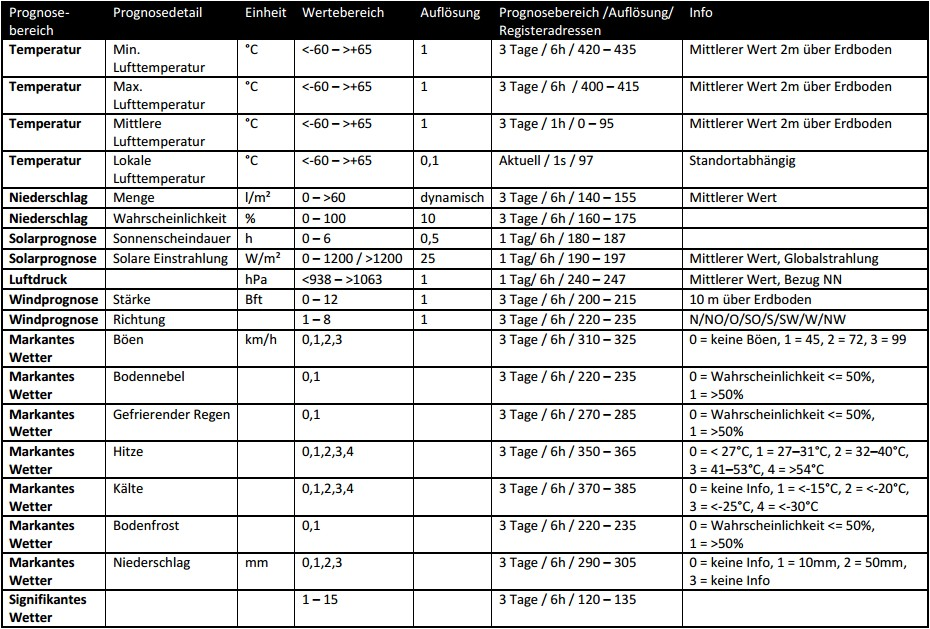
\includegraphics[scale=0.65]{weatherstation/TabDatenstruktur}
%\caption{Detailierte Datenstruktur der Wetterstation\cite[S. 17-26]{HKWDoc}}
%\label{fig:detaildatenstruktur}
%\end{figure}
\begin{table}[!b]
\rotatebox{90}{
\begin{minipage}[!b]{\textwidth}
\resizebox{18.9cm}{!}{ 
\rowcolors{1}{cyan}{white}
{
\setlength{\extrarowheight}{0.1cm}
\begin{tabular}[!b]{| p{2.5cm} | l | l | l | l | l | l | l | p{6.4cm} |}
\hline
\textbf{\parbox[t]{2.7cm}{Prognose-\\Bereich}} & \textbf{Prognosedetail} & \textbf{\parbox[t]{1.2cm}{Ein-\\heit}} & \textbf{Wertebereich} & \textbf{\parbox[t]{1.7cm}{Auf-\\lösung}} & \textbf{\parbox[t]{1.95cm}{Prognose-\\intervall}} & \textbf{\parbox[t]{1.9cm}{zeitliche\\Auflösung}} & \textbf{\parbox[t]{1.9cm}{Register-\\adresse}} & \textbf{Info}\\[1cm]
%\textbf{\parbox[t]{2cm}{Prognose-\\bereich}} & \textbf{Prognosedetail} & \textbf{Einheit} & \textbf{Wertebereich} & \textbf{Aufloesung} & \textbf{Prognoseintervall} & \textbf{zeitliche Aufloesung} & \textbf{Registeradresse} & \textbf{Info}\\[1cm]
\hline \hline
\hiderowcolors
Temperatur & Min. Lufttemperatur & $^\circ$C &  $<-60$ bis $>65$ & 1 & 3 Tage & 6h & 420 - 435 & Mittlerer Wert 2m über Erdboden\\
Temperatur & Max. Lufttemperatur & $^\circ$C &  $<-60$ bis $>65$ & 1 & 3 Tage & 6h & 400 - 415 & Mittlerer Wert 2m über Erdboden\\
Temperatur & Mittlere Lufttemperatur & $^\circ$C &  $<-60$ bis $>65$ & 1 & 3 Tage & 1h & 000 - 095 & Mittlerer Wert 2m über Erdboden\\
Temperatur & Lokale Lufttemperatur & $^\circ$C &  $<-60$ bis $>65$ & 1 & Aktuell & 1s & 097 & Standortabhängig\\
Niederschlag & Menge & l/m$^2$ &  0-60 & dyn. & 3 Tage & 6h & 140 - 155 & Mittlerer Wert\\
Niederschlag & Wahrscheinlichkeit & \% &  0 - 100 & 10 & 3 Tage & 6h & 160 - 175 & \\
Solarprognose & Sonnenscheindauer & h &  0 - 6 & 1 & 1 Tag & 6h & 180 - 187 & Mittlerer Wert\\
Solarprognose & Solare Einstrahlung & W/m$^2$ &  0 – 1200/$>1200$ & 25 & 1 Tag & 6h & 190 - 197 & Mittlerer Wert Globalstrahlung\\
Luftdruck & Min. Lufttemperatur & hPa &  $<938$ – $>1063$ & 1 & 1 Tag & 6h & 240 - 247 & Mittlerer Wert bezogen auf NN\\
Windprognose & Stärke & Bft &  0 - 12 & 1 & 3 Tage & 6h & 200 - 215 & Mittlerer Wert 10m über Erdboden\\
Windprognose & Richtung &  &  1 - 8 & 1 & 3 Tage & 6h & 220 - 235 & N/NO/O/SO/S/SW/W/NW\\
Markantes Wetter & Böen &  &  0,1,2,3 & 1 & 3 Tage & 6h & 310 - 325 & 0=keine Böen, 1=45km/h, 2=72km/h, 3=99km/h \\
Markantes Wetter & Bodennebel &  & 0,1 & 1 & 3 Tage & 6h & 250 - 265 & 0=Wahrscheinlichkeit$<=$50\%, 1=$>$50\%\\
Markantes Wetter & Gefrierender Regen &  & 0,1 & 1 & 3 Tage & 6h & 270 - 285 & 0=Wahrscheinlichkeit$<=$50\%,1=$>$50\%\\
Markantes Wetter & Hitze & $^\circ$C &  0,1,2,3,4 & 1 & 3 Tage & 6h & 350 - 365 & 0=$<$27$^\circ$C, 1=27–31$^\circ$C, 2=32–40$^\circ$C, 3=41–53$^\circ$C, 4=$>$54$^\circ$C\\
Markantes Wetter & Kälte & $^\circ$C &  0,1,2,3,4 & 1 & 3 Tage & 6h & 370 - 385 & 0=keine Info, 1=$<$-15$^\circ$C, 2=$<$-20$^\circ$C, 3=$<$-25$^\circ$C, 4=$<$-30$^\circ$C\\
Markantes Wetter & Bodenfrost &  &  0,1 & 1 & 3 Tage & 6h & 290 - 305 & 0=Wahrscheinlichkeit$<=$50\%, 1=$>$50\%\\
Markantes Wetter & Niederschlag &  &  0,1,2,3 & 1 & 3 Tage & 6h & 330 - 345 & 0=keine Info, 1=10mm, 2=50mm, 3=keine Info\\
Signifikantes Wetter &  &  & 1 - 15 & 1 & 3 Tage & 6h & 120 - 135 & 1=sonnig/klar, 2=leicht bewölkt, 3=vorwiegend bewölkt, 4=bedeckt, 5=Wärmegewitter, 6=starker Regen, 7=Schneefall, 8=Nebel, 9=Schneeregen, 10=Regenschauer, 11=leichter Regen, 12=Schneeschauer, 13=Frontengewitter, 14=Hochnebel, 15=Schneeregenschauer\\
\hline
\end{tabular}
}
}
\caption{Detailierte Datenstruktur der Wetterstation\cite[S. 17-26]{HKWDoc}}
\label{tab:detaildatenstruktur}
\end{minipage}
}
\end{table}
\FloatBarrier
\chapter{Das MODBUS Protokoll}
\begin{figure}[h]
\centering
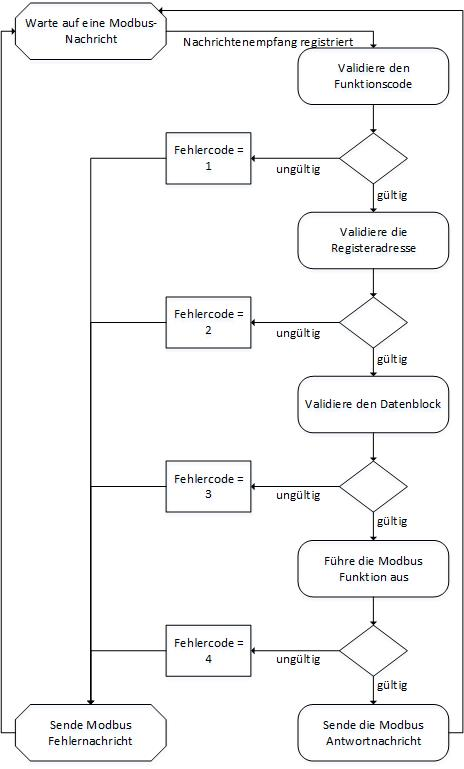
\includegraphics[scale=0.65]{modbus/modbustransdiag}
\caption{Ablaufdiagramm für die MODBUS Nachrichtenüberprüfung \cite[S. 9]{ModbusDoc}}
\label{fig:modbustransdiag}
\end{figure}
\newpage
\begin{figure}[hbtp]
\centering
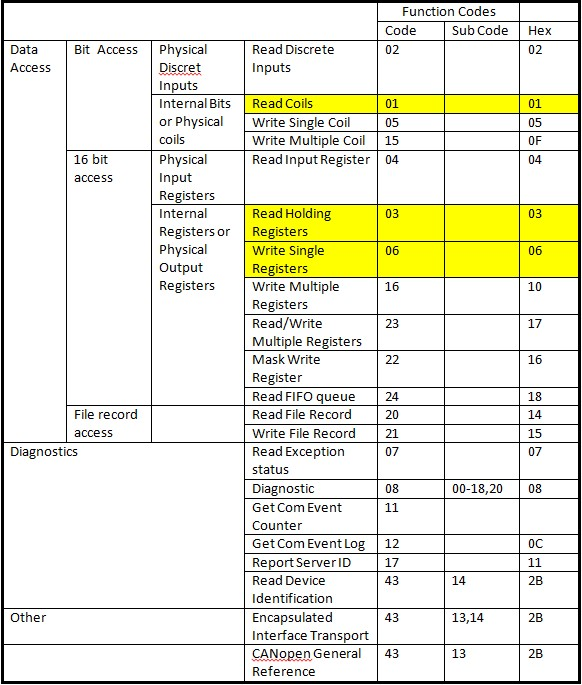
\includegraphics[scale=0.65]{modbus/fcodetab}
\caption{Übersicht der zur Verfügung stehenden Funktionscodes in MODBUS \cite[S. 11]{ModbusDoc}}
\label{fig:fcodetab}
\end{figure} 
\chapter{Hilfsfunktionen}
\section{read\_com\_set}\label{sec:readcomset}
Die Funktion \textsf{read\_com\_set} ermöglicht es auch außerhalb des Funktionsaufrufs von \textsf{forecast\_data} Parameter der Wetterstation abzurufen sofern eine serielle Schnittstelle besteht. Neben dem Abruf nur eines Parameters, können auch mehrere Parameter gleichzeitig in einem Cell-Array übergeben werden. Die Ausgabe der abgerufenen Werte erfolgt dabei in der Reihenfolge der angefragten Parameter. Da die Funktion \textsf{send\_and\_receive\_data} hier keine Daten interpolieren oder abspeichern muss, werden die Parameter für Längen- und Breitengrad, Verbindungsqualität, lokaler Temperatur und Pfadangabe des Speicherortes nicht benötigt. 
\lstinputlisting[firstline=1, lastline=54]{programm/readcomset.m}
\section{write\_com\_set}\label{sec:writecomset}
Übergabeparameter für diese Funktion sind die Slave ID, der zu schreibende Wert in dezimal Format und die Spezifizierung der Adresse im String Format. Der Zähler \textit{cnt} dient zur Initialisierung des while-Schleifendurchlaufs. Siehe hierzu Kapitel~\ref{sec:rxdatenverarbeitung} auf Seite~\pageref{sec:rxdatenverarbeitung}.
Der Inputwert wird in hex umgerechnet, danach wird die Registeradresse ermittelt, die PDU gebildet und über die serielle Schnittstelle geschickt.
\lstinputlisting{programm/writecomset.m}
\section{stop\_timer}\label{sec:stoptimer}
Die Funktion \textsf{stop\_timer} meldet dem Nutzer das Ende des Timer Objektes, löscht es, speichert den Datencontainer mit den Langzeitdaten ab und schließt die serielle Schnittstelle. Vorteil dieser Funktion ist es, sobald ein Fehler in der forecast Funktion auftritt, wird zumindest der Datencontainer immer noch gesichert.
\lstinputlisting{programm/stoptimer.m}
\section{get\_reg\_address}\label{sec:getregadd}
Die Funktion erhält einen String mit der Information ob es sich um eine Abfrage für die Einstellungsparameter oder Wetterdaten der Wetterstation handelt. Da das Register mit den Adressen in einem struct angelegt wurde, kann man die gesuchte Adresse einfach durch Vorgabe der Zweigpunkte mit dem Befehl \textsf{getfield} in dieser Struktur abrufen. Man hätte die Registeradressdaten auch in einem Database anlegen können, aber auch hier hat ein Test gezeigt, dass der Abruf aus der Struktur ein bisschen schneller ist. Schließlich muss nicht immer wieder die komplette Database durchsucht werden. 
\lstinputlisting[firstline=1, lastline=59]{programm/getregaddress.m}
\section{reg\_num}\label{sec:regnum}
Es erfolgt die Berechnung der Anzahl an Registeradressen. Sind die Adressen gleich würde die Differenz 0 ergeben. Daher wird zum Ergebnis der Subtraktion eine 1 addiert.
\lstinputlisting{programm/regnum.m}
\section{format\_modbus\_msg}\label{sec:formatmodbusmsg}
Die Funktion \textsf{format\_modbus\_msg} transformiert den n-Byte großen String der MODBUS-Nachricht in einen n-zeiligen Vektor mit dezimalen Werten.
\lstinputlisting{programm/formatmodbusmsg.m}
\section{fcode\_check}\label{sec:fcodecheck}
Es wird lediglich überprüft, ob der Funktionscode den Wert 1, 3 oder 6 hat. Ist dies nicht der Fall, wird das Flag \textit{fcode\_error} auf 1 gesetzt.
\lstinputlisting{programm/fcodecheck.m}
\section{MESZ\_calc}\label{sec:meszcalc}
Die Berücksichtigung der MESZ spielt vor allem für die Berechnung des Sonnenauf- und Sonnenuntergangs eine Rolle. Aber auch bei der Erstellung des Zeitstempels für den Zeitpunkt des Datenabrufs. Hierbei wird einfach überprüft ob das aktuelle Datum im Intervall für die Sommerzeit liegt oder nicht. Entsprechend wird das Flag ausgegeben.
\lstinputlisting{programm/MESZcalc.m}
\section{res\_factor}\label{sec:resfactor}
Da die Ausgangsdaten selbst in unterschiedlicher Auflösung vorliegen, muss zur Berechnung der Anzahl interpolierter Werte ein Faktor verwendet werden. Dieser ergibt sich aus der zu Grunde liegenden zeitlichen Auflösung geteilt durch die gewünschte zeitliche Auflösung.
\lstinputlisting{programm/resfactor.m}
\section{utc2date}\label{sec:utc2date}
Diese Funktion wurde so geschrieben, dass sie Eingabevektoren verarbeiten kann. Ohne diese Maßnahme hätte bei der Interpolation eine for-Schleife für die Berechnung der Start- und Stopzeitpunkte des Gültigkeitsintervalles der Daten in normalem Zeitformat verwendet werden müssen. Ein Test der Laufzeitverbesserung ergab 12 Sekunden für eine for-Schleife. Der hier verwendete Algorithmus entspricht dem im Minix Source Code verwendeten Algorithmus.\cite{utc2date}
\lstinputlisting{programm/utc2date.m}
\section{tvector}\label{sec:tvector}
\lstinputlisting{programm/tvector.m}
\section{date2utc}\label{sec:date2utc}
Der hier verwendete Algorithmus entspricht der Berechnungsvorschrift des IEEE.\cite[S. 113]{date2utc}
\lstinputlisting{programm/date2utc.m}
\section{data\_mult}\label{sec:datamult}
Laut Spezifikation des Herstellers\cite[S. 19-20]{HKWDoc} müssen die Werte für die Niederschlagsmenge und die Sonnenscheindauer durch 10 geteilt werden, um die Einheiten l/m² und h zu erhalten.
\lstinputlisting{programm/datamult.m}
\section{diurnal\_var}\label{sec:diurnalvar}
Der Algorithmus für die Berechnung des Sonnenauf- und Sonnenuntergangzeitpunktes wurde dem Kapitel 2.2 \enquote{Astronomische Gegebenheiten} entnommen. \cite{Wagner.2006}
\lstinputlisting{programm/diurnalvar.m}
\section{neg\_val\_corr}\label{sec:negvalcorr}
Funktionsinput sind das Prognosedetail oder der Prognosebereich, die interpolierten Werte und die dazugehörigen Messzeitpunkte. Abhängig von den übergebenen Wetterdaten wird das übergebene Zeitintervall der Messpunkte entweder aufgeteilt oder nicht. Für die Daten der Solarleistung, werden Zeitbereiche gebildet, die vor Sonnenauf- und nach Sonnenuntergang liegen, bzw. dazwischen. Werte egal ob positiv oder negativ, die nach oder vor Sonnenauf- bzw. Sonnenuntergang liegen werden zu Null gesetzt. Werte die dazwischen liegen und negativ sind werden zu Null gesetzt. Für die Niederschlagsmenge und Windstärke werden alle negativen Werte zu Null gesetzt.
\lstinputlisting{programm/negvalcorr.m}
\section{crc\_check}\label{sec:crccheck}
Der CRC Check zerlegt die empfangene Nachricht des Slaves. Von Interesse ist nur der Teil der Nachricht ohne CRC Summe \textit{size(rxdata,1-2)}. Für jedes Byte wird die Dezimalzahl in eine Hexzahl konvertiert und zur MODBUS Nachricht in Hexformat zusammengesetzt. Danach wird die Funktion \textsf{crc\_calc} verwendet um deren Ergebnis mit dem übermittelten CRC Wert zu vergleichen.
\lstinputlisting{programm/crccheck.m}
\chapter{Abkürzungsverzeichnis}
\begin{acronym}
\setlength{\parskip}{0ex}
\setlength{\itemsep}{1ex}
 \acro{ADU}{Application Data Unit}
 \acro{Bft}{Beaufort}
 \acro{C}{Celsius}
 \acro{COM}{Communication}
 \acro{CRC}{Cyclic Redundancy Check}
 \acro{DWD}{Deutscher Wetterdienst}
 \acro{EMU}{Energy Management Unit}
 \acro{EV}{Electric Vehicle}
 \acro{FSK}{Frequency Shift Keying}
 \acro{GmbH}{Gesellschaft mit beschränkter Haftung}
 \acro{h}{Stunde}
 \acro{hPa}{Hektopascal}
 \acro{HEMS}{Home Energy Management System}
 \acro{H-Byte}{High-Byte}
 \acro{ID}{Identifkationsnummer}
 \acro{int8}{8 Bit-Integer}
 \acro{IP}{Internet Protocol}
 \acro{I/O}{Input/Output}
 \acro{LMU}{Ludwig-Maximilians-Universität}
 \acro{L-Byte}{Low-Byte}
 \acro{N}{Nord}
 \acro{NN}{Normal Null Meeresspiegel}
 \acro{NO}{Nordost}
 \acro{NW}{Nordwest}
 \acro{O}{Osten}
 \acro{OSI}{Open Systems Interconnection}
 \acro{PDU}{Protocol Data Unit}
 \acro{RMSE}{Root mean square error}
 \acro{RS}{Recommended Standard}
 \acro{RTU}{Remute Terminal Unit}
 \acro{rx}{Empfänger}
 \acro{TCP}{Transmission Control Protocol}
 \acro{S}{Sueden}
 \acro{SO}{Suedost}
 \acro{SW}{Suedwest}
 \acro{W}{Westen}
\end{acronym}
